\section{Excerpts from MINA commit comments w.r.t. the Strategy pattern}
\label{sec:strategy_motivation}
For the analysis of the Strategy pattern in section \ref{sec:pattern_analysis}, we based our conclusions on the analysis of 42 Strategy pattern instances related to the \texttt{IOService} scope. In this section, we present the categorized motivations for removing the Strategy pattern that we have identified during our analysis:
\begin{enumerate}
    \item Solving issues:
  
            \begin{enumerate}
                \item \textit{"DIRMINA-209 - The number of processors for socket connectors and acceptors can be specified via a cxtor parameter. By default, connectors and acceptors each use their own processor.
                Additionally, the delegates have been removed helping to simplify the code."}
                \item \textit{"Resolved issue: DIRMINA-162"}
                \item \textit{"DIRMINA-267 - Allow usage of an Executor for launching threads in processors/acceptors"}
                \item \textit{"Resolved issue: DIRMINA-290 (Make IoService (IoConnector and IoAcceptor) manage only one service.)"}
                \item \textit{"Fixed compilation warnings"}
                \item \textit{"Related issue: DIRMINA-341 (Allow binding multiple SocketAddresses per IoAcceptor.)
                * Added IoAcceptor.localAddresses property"}
                \item \textit{"Resolved issue: DIRMINA-449 (Improve current JMX integration code using new statistical properties.)"}
                \item \textit{"Fixed some Sonar warnings"}
                \item \textit{"Removing cyclic dependencies..."}
                \item \textit{"* Resolved issue: DIRMINA-432 (IoService method for writing Object to all the managed IoSession)"}
                \item \textit{"Removed the ServerSocket creation and socket connection in the Socket/DatagramConfigImpl classes : it breaks badly in an applet or on Vista."}
            \end{enumerate}
    
    
    \item Additions, updates or improvements to the code base:
        
                \begin{enumerate}
                    \item \textit{" Added IoSessionConfig and its implementations
                    * Added IoServiceConfig and its implementations
                    * Added IoAcceptorConfig and its implementations
                    * Added IoConnectorConfig and its implementations
                    * Replaced all transport-type specific properties with the Config classes above"}
                    \item \textit{"Updated Spring integration code to work with the new IoService/IoServiceConfig design."}
                    \item \textit{"JMX integration module for MINA"}
                    \item \textit{"StatCollector used for collecting IoSession throughput values"}
                    \item \textit{"* Added BaseIoSession.getServiceAddress() * Optimized DatagramSessionImpl"}
                    \item \textit{"* Added IoServiceMetadata.hasFragmentation() * Added DefaultIoServiceMetadata"}
                    \item \textit{"initial check-in.  much is left to do in the commenting section.  This will at least get the ball rolling and allow others to make updates."}
                    \item \textit{"* Updated POM.xmls
                    * renamed protocol-client-http to protocol-http-client
                    * renamed protocol-server-http to protocol-http-server"}
                    \item \textit{"* Added AbstractIoProcessor; extracted from SocketIoProcessor
                    * Rewrote SocketIoProcessor to use AbstractIoProcessor
                    * Added IoSessionConfig properties
                    ** readBufferSize
                    ** minReadBufferSize
                    ** maxReadBufferSize"}
                    \item \textit{"* Added IoService interfaces to transport.socket and made the classes in transport.socket.nio implement it."}
                    \item \textit{"Applied Generics to IoProcessor"}
                    \item \textit{"Removed java5 module and backport-util-concurrent dependency"}
                \end{enumerate}
        
    \item Re-namings/refactorings/ or changes for documentation purposes:
        
            
                \begin{enumerate}
                    \item \textit{"Renamed IoSessionManager to IoService, which is shorter."}
                    \item \textit{"* Code cleanup"}
                    \item \textit{"* Renamed Base* to Abstract* which sounds more familiar to most developers
                    * Renamed DelegatedIoAcceptor to IoAcceptorWrapper and DelegatedIoConnector to IoConnectorWrapper respectively
                    * Renamed SessionIdleStatusChecked to IdleStatusChecker to make its name get aligned with IdleStatus type
                    * Renamed SessionLog to IoSessionLogger to make its name get aligned with IoSession type and SLF4J Logger type"}
                    \item \textit{"* Moved classes in transport.vmpipe.support to transport.vmpipe* Made IoSessionConfig implementations package-private"}
                    \item \textit{"renamed the modules to mina-<module> (all but distribution)"}
                \end{enumerate}

\end{enumerate}

\begin{figure}[H]
    \centering
    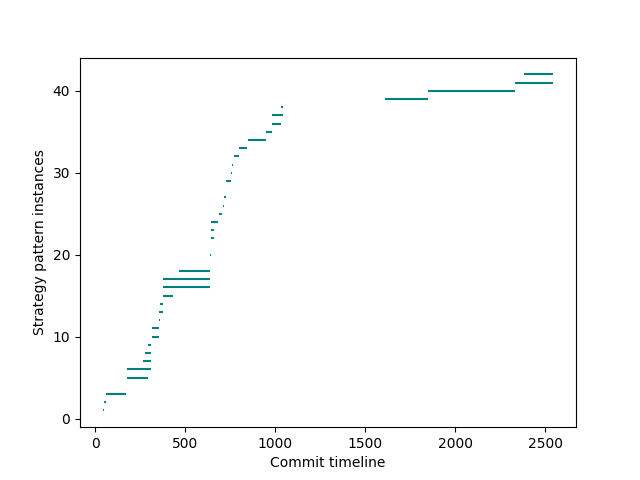
\includegraphics[width = 0.7\textwidth]{images/strategy_timeline.png}
    \caption{Depiction of the Strategy pattern timeline within the \texttt{IOService} scope; as can be seen, a removal is generally followed by the introduction of a new instance of the Strategy pattern; Pinot does not identify any Strategy pattern instance between coomit \#1041 and \#1610.}
    \label{fig:strategy_timeline}
\end{figure}